%! Author = Jan
%! Date = 13.05.2022

\section*{Defusing Bombs}
A bomb will explode when its countdown timer reaches 0:00 or when too
many strikes have been recorded. The only way to defuse a bomb is to disarm
all of its modules before its countdown timer expires.

\begin{figure}[h]
  \centering
  \caption*{Example Bomb}
  \begin{minipage}{.4\textwidth}
    \centering
    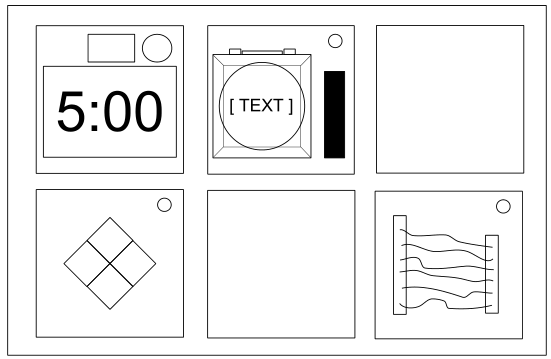
\includegraphics[height=4.5cm]{modules/0_explanation/bomb_front}
    \caption*{Front}
    \label{fig:sub1}
  \end{minipage}%
  \begin{minipage}{.3\textwidth}
    \centering
    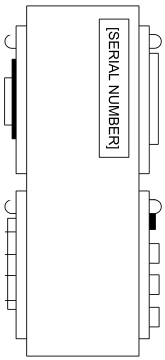
\includegraphics[height=4.5cm]{modules/0_explanation/bomb_side}
    \caption*{Side}
    \label{fig:sub2}
  \end{minipage}
  \label{fig:example_bomb}
\end{figure}

\subsection*{Modules}
Each bomb will include one or several modules that must be disarmed. Each
module is discrete, but some modules require to be solved before others.


Instructions for disarming modules can be found in Section 1.
"Needy" modules present a special case and are described in Section 2.

\subsection*{Strikes}
\begin{wrapfigure}[7]{r}{0.2\textwidth} %this figure will be at the right
  \vspace{-2\baselineskip}
  Strike Indicator
  \centering
  
\includegraphics[height=3.5cm]{modules/0_explanation/strike}
  \label{fig:Strikes}
\end{wrapfigure}
When the Defuser makes a mistake the bomb will record a strike
which will be displayed on the indicator above the countdown
timer. Bombs with a strike indicator will explode upon the
third strike. The timer will begin to count down faster after
a strike has been recorded.

If no strike indicator is present above the countdown timer,
the bomb will explode upon the first strike, leaving no room
for error.

\subsection*{Gathering Information}
Some disarming instructions will require specific information about the
bomb, such as the serial number. For detailed descriptions see the next
page "On the Subject of Edgework".

\clearpage

\section*{On the Subject of Edgework}\label{sec:on-the-subject-of-edgework}
The term edgework describes all kinds of widgets that can be found on the
side casings of a bomb. The different kinds and their meanings are
described in the following sections. Many modules ask for specific
information about the edgework.

\subsection*{Serial Number}\label{subsec:serial-number1}
\begin{wraptable}[4]{r}{0.22\textwidth}
  \vspace{-2\baselineskip}
  \centering
  \begin{tabular}{| c |}
    \hline
    \color{white}
    \cellcolor{red}
    Serial \#
    \\ \hline
    \marginbox{0.3cm}{\huge{I6K3NP}}
    \\ \hline
  \end{tabular}\label{tab:serial_section}
\end{wraptable}
The serial number is a code of six symbols and is made up
of uppercase letters and digits. There is always at least
one digit in the serial number. A zero has a diagonal line
crossing through it, while the letter O does not.

\subsection*{Indicator Lights}\label{subsec:indicator-lights}
\begin{wrapfigure}[3]{r}{0.251\textwidth} %this figure will be at the right
  \vspace{-2\baselineskip}
  \centering
  \begin{tikzpicture}
    \coordinate (dm1) at (2,0.6);
    \coordinate (dm2) at (-2,-0.6);
    \coordinate (dm3) at (-1.5,0);
    \coordinate (dm4) at (-1,0);
    \coordinate (dm5) at (1.8,0.6);
    \coordinate (dm6) at (0,0);
    \node[rectangle,draw,fill=red] [fit = (dm1) (dm2)] (bx4) {};
    \node[circle,draw=lightgray,line width=2.5,fill=white] [fit = (dm3) (dm4)] (circle) {};
    \node[rectangle,draw,minimum, fill=black] [fit = (dm5) (dm6)] (bx4) [right=0.4cm of circle] {};
    \node[align=center,font=\large,color=white] at (bx4.center) {BOB};
%        \draw [black, fill=red, align=center] (2,1) rectangle (-1,-1) node [black] {\centering Start}; % Draws a rectangle
  \end{tikzpicture}
  \label{fig:lights}
\end{wrapfigure}
Indicator lights can be lit or unlit and are accompanied
by a three letter code. Common codes include:

BOB, CAR, CLR, FRK, FRQ, IND, MSA, NSA, SIG, SND, TRN

\subsection*{Batteries}\label{subsec:batteries}
\begin{wraptable}[4]{r}{0.28\textwidth}
  \vspace{-2\baselineskip}
  \begin{tabular}{| c | c |}
    \hline
    \cellcolor{lightgray} AA &
    \cellcolor{lightgray} D
    \\ \hline
    
\includegraphics[width=1.8cm]{modules/0_explanation/battery_aa} &
    \marginbox{0.1cm}{
\includegraphics[width=1.8cm]{modules/0_explanation/battery_d}}
    \\ \hline
  \end{tabular}\label{tab:batteries}
\end{wraptable}
There are two types of batteries that can occur on a
bomb. They are always placed in battery holders. A
holder contains two AA batteries or one D battery.
For some modules the number of holders is relevant.

\subsection*{Ports}\label{subsec:ports}
There are six types of ports that can occur on a bomb. Note that the stereo
RCA port consists of two individual sockets, one white and one red, but
both together count as a single port only.
\begin{table}[h]
  \centering
  \begin{tabular}{|
      >{\centering\arraybackslash}p{0.3\textwidth} |
      >{\centering\arraybackslash}p{0.3\textwidth} |
      >{\centering\arraybackslash}p{0.3\textwidth} |}
    \hline
    \cellcolor{lightgray} DVI-D &
    \cellcolor{lightgray} Parallel &
    \cellcolor{lightgray} Serial \\ \hline
    \vspace{0cm}
    
\includegraphics[height=0.8cm,valign=b]{modules/0_explanation/ew_dvi-d} &
    \vspace{0cm}
    
\includegraphics[height=0.8cm,valign=b]{modules/0_explanation/ew_parallel} &
    \vspace{0cm}
    
\includegraphics[height=0.8cm,valign=b]{modules/0_explanation/ew_serial} \\ \hline
  \end{tabular}\label{tab:portsA}
\end{table}
\begin{table}[h]
  \centering
  \begin{tabular}{|
      >{\centering\arraybackslash}p{0.3\textwidth} |
      >{\centering\arraybackslash}p{0.3\textwidth} |
      >{\centering\arraybackslash}p{0.3\textwidth} |}
    \hline
    \cellcolor{lightgray} PS/2 &
    \cellcolor{lightgray} RJ-45 &
    \cellcolor{lightgray} Stereo RCA \\ \hline
    \vspace{0cm}
    
\includegraphics[height=0.8cm]{modules/0_explanation/ew_ps2} &
    \vspace{0cm}
    
\includegraphics[height=0.8cm]{modules/0_explanation/ew_rj-45} &
    \vspace{0cm}
    
\includegraphics[height=0.8cm]{modules/0_explanation/ew_stereo} \\ \hline
  \end{tabular}\label{tab:portsB}
\end{table}^
